% mnras_template.tex
%
% LaTeX template for creating an MNRAS paper
%
% v3.0 released 14 May 2015
% (version numbers match those of mnras.cls)
%
% Copyright (C) Royal Astronomical Society 2015
% Authors:
% Keith T. Smith (Royal Astronomical Society)

% Change log
%
% v3.0 May 2015
%    Renamed to match the new package name
%    Version number matches mnras.cls
%    A few minor tweaks to wording
% v1.0 September 2013
%    Beta testing only - never publicly released
%    First version: a simple (ish) template for creating an MNRAS paper

%%%%%%%%%%%%%%%%%%%%%%%%%%%%%%%%%%%%%%%%%%%%%%%%%%
% Basic setup. Most papers should leave these options alone.
\documentclass[fleqn,usenatbib,letters]{mnras}%added "letters", a4paper is default

% MNRAS is set in Times font. If you don't have this installed (most LaTeX
% installations will be fine) or prefer the old Computer Modern fonts, comment
% out the following line
%\usepackage{newtxtext,newtxmath}
% Depending on your LaTeX fonts installation, you might get better results with one of these:
\usepackage{mathptmx}
%\usepackage{txfonts}

% Use vector fonts, so it zooms properly in on-screen viewing software
% Don't change these lines unless you know what you are doing
\usepackage[T1]{fontenc}
\usepackage{ae,aecompl}


%%%%% AUTHORS - PLACE YOUR OWN PACKAGES HERE %%%%%

% Only include extra packages if you really need them. Common packages are:
\usepackage{graphicx}	% Including figure files
\usepackage{amsmath}	% Advanced maths commands
\usepackage{amssymb}	% Extra maths symbols
\usepackage{cases}  %define a step function

%%%%%%%%%%%%%%%%%%%%%%%%%%%%%%%%%%%%%%%%%%%%%%%%%%

%%%%% AUTHORS - PLACE YOUR OWN COMMANDS HERE %%%%%


%%%%%%%%%%%%%%%%%%%%%%%%%%%%%%%%%%%%%%%%%%%%%%%%%%

%%%%%%%%%%%%%%%%%%% TITLE PAGE %%%%%%%%%%%%%%%%%%%

% Title of the paper, and the short title which is used in the headers.
% Keep the title short and informative.
\title[]{No flaring star-planet interactions in AU Mic TESS observations}

% The list of authors, and the short list which is used in the headers.
% If you need two or more lines of authors, add an extra line using \newauthor
\author[E. Ilin et al.]{
E. Ilin$^{1,2}$,\thanks{E-mail: eilin@aip.de}
K. Poppenhaeger$^{1,2}$,
\\
% List of institutions
$^{1}$Leibniz-Institute for Astrophysics Potsdam (AIP), An der Sternwarte 16, 14482 Potsdam, Germany\\
$^{2}$Institute for Physics and Astronomy, University of Potsdam, Karl-Liebknecht-Str. 24/25, 14476 Potsdam, Germany
}

% These dates will be filled out by the publisher
\date{Accepted XXX. Received YYY; in original form ZZZ}

% Enter the current year, for the copyright statements etc.
\pubyear{2020}

% Don't change these lines
\begin{document}
\label{firstpage}
\pagerange{\pageref{firstpage}--\pageref{lastpage}}
\maketitle

% Abstract of the paper
\begin{abstract}
Planets that move in close orbits around magnetically active stars can interact with their magnetic fields in a way that modulates the star's activity. This modulation in phase with the planet's orbit, such as enhanced X-ray activity, chromospheric spots, radio emission, or flares, is considered the clearest sign of magnetic star-planet interaction (SPI). However, the magnitude of this interaction is poorly constrained, and the intermittent nature of the interaction is a challenge for observers. 

AU Mic is an early M dwarf, and the most actively flaring planet host detected to date. Its innermost companion, AU Mic b, a warm Neptune in a 8.6 day orbit is a promising target for magnetic SPI observations. In this study, we used optical light curves of AU Mic obtained by the Transiting Exoplanet Survey Satellite to search for signs of flaring SPI with AU Mic b using a customized Anderson-Darling test. 

In the about 50 days of observations the distribution of flares with orbital, rotational, and synodic phases was consistent with intrinsic stellar flaring. We discuss possible physical and observational reasons for the absence of flaring SPI signal in the light curves. We conclude that, if flaring SPI signal is present but weak, continued monitoring of AU Mic by mission like TESS and PLATO will favor the detection of flaring SPI with orbital phase.

\end{abstract}

% Select between one and six entries from the list of approved keywords.
% Don't make up new ones.
\begin{keywords}
stars: individual: AU Mic -- planet-star interactions -- stars: flare -- planets and satellites: individual: AU Mic b
\end{keywords}

%%%%%%%%%%%%%%%%%%%%%%%%%%%%%%%%%%%%%%%%%%%%%%%%%%
%
%-------------------------------------------------------------------

\section{Introduction}

Flares are electromagnetic explosions in the stellar corona that are driven by the dynamics of the surface magnetic fields~\citep{benz2010}. They can be triggered intrinsically by the star in isolation, but also by magnetic star-planet interaction (SPI).

In SPI flares, the event is induced by the re-connection of stellar and planetary magnetic field lines~\citep{saur2013,lanza2018close-by,fischer2019}. For this to occur, the planet must revolve around the star in close orbit, so that it moves within the stellar Alfv\'en zone for at least a fraction of its orbit. When the planet is within the Alfv\'en zone, the magnetic field and the energy transported along the field lines as particles or waves can fall back on to the star, whereas outside of it it would be carried away by the stellar wind pressure. 


%When re-connection between star and planet occurs, the energy channelled back into the stellar atmosphere can create an activity hot spot (XXXX Halpha? Xray?) trigger a flare. The footpoint of the connecting field line is expected to move with the planetary orbit (but need not neccessarily be the sub-planetary point).

Several studies of individual systems with close-in and eccentric Hot Jupiters report excess flaring in phase with the planet or close to periastron~\citep{shkolnik2005,pillitteri2011,maggio2015}, but in light of many non-detections of excess flares in similar systems~\citep{figueira2016, fischer2019}, flaring SPI remains an elusive phenomenon. 

One interpretation is that the interaction is so weak and intermittent that the system has to be observed for many orbits of the interacting planet before SPI flares become measurable against the background of intrinsic flares~\citep{shkolnik2008,lanza2009, saur2013,strugarek2015}.

Recently, AU Mic, an M0-M1~\citep{pecaut2013,gaidos2014} pre-main sequence dwarf star has been shown to be a promising candidate for magnetic SPI with its innermost planet~\citep{kavanagh2021}. AU Mic is a member of the $\beta$ Pic young moving group, which is $16-29$ Myr old~\citep{malo2014,binks2014,mamajek2014,bell2015,binks2016,shkolnik2017,miretroig2020}. %Based on its lithium abundance, AU Mic could be a few Myr older than the average group member~\citep{malo2014}. 
%Its rotation period of about $4.862$ d~\citep{plavchan2020, martioli2021} was determined from photometry obtained by the Transiting Exoplanet Survey Satellite~\citep[TESS,][]{ricker2014}.

AU Mic rotates at a $4.862$ d period; it shows strong solar-like differential rotation; possesses a strong, mostly poloidal large-scale magentic field of $>400$ G; and several activity indicators vary in phase with the star's latitude-dependent rotation periods~\citep{klein2021}. Optical light curves obtained by the Transiting Exoplanet Survey Satellite~\citep[TESS,][]{ricker2014} confirm previous observations~\citep{katsova1999, robinson2001, redfield2002} that AU Mic is actively flaring~\citep{martioli2021new}.
%Spectral type tends to agree on M1, but effective temperature is lower in Plavchan et al. (2009)

AU Mic b is a Neptune-sized planet ($R_p = 4.3R_{Earth}$) that was first discovered using TESS photometry~\citep{plavchan2020} with an orbital period of $8.463$ d~\citep{plavchan2020,martioli2021new}. %A magnetic interaction between star and planet can not only trigger flares, but also enhance X-ray activity and produce chromospheric hot spots~\citep{lanza2009}%, but the exact form and intesity of the interaction is difficult to assess even for individual stars~\citep{strugarek2019} 
\citet{kavanagh2021} predict magnetic SPI with AU Mic b to be observable in the radio regime, a signal indicative of a phenomenon similar to auroral flares observed in the Jupiter-Io system. Since AU Mic is the most actively flaring star among all currently known exoplanet hosts (Ilin et al. in prep.), we may expect SPI flares to also be triggered more readily by AU Mic b than in less active star-planet systems. 

In this work, we searched the TESS light curves of AU Mic for signs of flaring SPI. We present our light curve de-trending and flare finding method in Section \ref{sec:detrendfind}, and present the resulting flare catalog in Section \ref{sec:flarecatalog}. In Section \ref{sec:phases}, we show how we can combine flare samples from general time series measurements into a homogeneous data set, and apply this method to test whether flaring SPI signal is present in the TESS observations. The main result is shown in Table~\ref{tab:pvals}. We discuss our results and present our conclusions in Sections~\ref{sec:discussion} and \ref{sec:conclusions}.


\section{TESS photometry}
The Transiting Exoplanet Survey Satellite~(TESS,~\citealt{ricker2014}) is an all-sky mission that began operations in 2018, and completed its first full sky scan in April 2020. It is still observing at the time of writing, collecting nearly continuous photometric times series in the 600-1000 nm band for $\sim 27$ d in each observing Sector. About $200\,000$ stars have been observed in 2 min cadence in the first two years of operations with about 20000 targets per Sector. Out of these, from Sector 27 on, 1000 targets were observed at even higher 20 s cadence.

AU Mic was observed in Sector 1 and 27 in 2 min cadence, and in Sector 27 in 20 s cadence. The light curves reveal strong rotational variability from starspots, vigorous flaring and show transits of two planets, AU Mic b~\citep{plavchan2020,martioli2021new} and AU Mic c~\citep{martioli2021new}.
% 20000 per sector does not add up, because of stars observed in multiple sectors, the 20000 and 1000 figures can be found here: https://tess.mit.edu/observations/target-lists/
% extended TESS mission https://heasarc.gsfc.nasa.gov/docs/tess/extended.html

\section{Light curve de-trending and flare finding}
\label{sec:detrendfind}
Stellar light curves are time series of flux measurements that vary due to both astrophysical and instrumental effects. Flares are only one of many phenomena like spot variability, transits, eclipses, bursts and dips that can be detected in the data. Accurate automated flare detection algorithms are still challenging to design~\citep{vida2021}, not least due to this intrinsically heterogeneous morphology of light curves. We applied an iterative three-step algorithm to remove all but the variations caused by flares, and derive a realistic noise estimate (Section~\ref{sec:detrend}), then used a two-step $\sigma$-clipping procedure to mark flare candidates and derive their properties~(Section~\ref{sec:flarefind}), and present the resulting flare catalog in Section~\ref{sec:flarecatalog}.

\subsection{De-trending}
\label{sec:detrend}
The light curves were de-trended in three steps, each of which removed variability on decreasing time scales while preserving the flare signal. Typical flare times range from a few minutes to a few hours, and rarely exceed one day in duration. Most stellar variability occurs on longer time scales, except for ultrafast rotational variability in some stars~(Ilin+2021, submitted). The following method was designed with a broad spectrum of Kepler~\citep{borucki2010} and TESS light curve types in mind. %Because AU Mic is extraordinarily active, we mark the adjustments made to accomodate that with comments in parentheses. 

First, we fit and subtract a third order spline function that goes through the start and end of any light curve portion that has no gaps longer than 2 h, and through an averaged flux point every 6 h (30 h for stars that are less variable than AU Mic) inbetween. This step removes long term trends as well as starspot variability on time scales of seveal days. If the light curve portion is shorter than 5 d, this step is skipped. 

Second, we iteratively remove strong periodic signal on time scales between 2 h and 5 d from the light curve. Each iteration first masks outlier points using a padded sigma-clipping procedure. For this step, single outliers above $3.5 \sigma$ are masked as pure outliers, and series of $n>1$ data points above $3.5 \sigma$ are masked as flare candidates or other extended outliers and padded with rounded $\sqrt{n}$ masked points before the outliers to capture slow rise phases, and rounded $2\sqrt{n}$ after the series to capture a potential extended decay phase that flares often display. Then we calculate a Lomb-Scargle periodogram for the light curve, and perform a least-square fit with a cosine function using the dominant frequency in the periodogram as a starting point. The cosine fit is then subtracted from the light curve. We iterate five times or until the dominant peak's signal-to-noise ratio drops below 1. 

As a third step, we again apply the padded outlier clipping, and smooth any remaining variability that is not sinusoidal, first with a 6 h and then with a 3 h window 3rd order Savitzky-Golay~\citep{savitzky1964} filter implemented in \texttt{scipy} as \texttt{signal.savgol\_filter}.

These three steps can sometimes overfit the very edges of the light curve, leaving small exponential drops or rises in the flux that affect the quiescent flux level calculation and/or produce false positive flare detections. If the first or the last data point is a $1\sigma$ outlier in the de-trended light curve, we fit an exponential growth or decay function to these fringes.

Finally we estimate the noise in the de-trended light curve using a rolling standard deviation with a 2 h window after padding outliers in the aforementioned way, but now above $1.5 \sigma$ ($2.5 \sigma$ for light curves with lower activity). We interpolated the masked outliers to arrive at a noise in the flare regions that is informed by the flux uncertainty in an adjacent light curve portion.

The result for the light curve in Sector 1 is shown in Fig.~\ref{fig:illustrate_detrend}. The method was inspired by the iterative approach in~\citet{davenport2016} who searched the entire Kepler catalog for flares. We tested our approach on a variety of synthetic and real light curves in the TESS and Kepler archives, so that it can be applied directly to a larger sample.

We provide an example script that shows how to use this method with Kepler and TESS short cadence light curve with \texttt{AltaiPony}.

\subsection{Flare finding}
\label{sec:flarefind}
We searched the de-trended light curves for flare candidates. For this, we first find an iterative median, and then apply the threshold method introduced by~\citep{chang2015} that requires three consecutive positive outliers $3 \sigma$ above median for a candidate detection. To these data points we then add subsequent data points until one of them falls below a $2 \sigma$ above median threshold in order not to cut off detectable parts of the flare decay phase. This series of data points is then flagged as a flare candidate. For each flare, the pipeline returns the flare start and end points, duration, amplitude, and equivalent duration ($ED$) with uncertainties. The $ED$ is the integrated flare flux $F_{flare}$ divided by the median quiescent flux $F_0$ of the star, integrated over the flare duration~\citep{gershberg1972}:
\begin{equation}
\label{eq:ED}
ED=\displaystyle \int \mathrm dt\, \frac{F_{flare}(t)}{F_0}.
\end{equation}


We tested our flare-finding procedure on a range of both real and synthetic light curves that covers several typically observed spot-induced variability signal patterns, and that contains flare signatures between ones that barely exceed the detection threshold to the largest flares we typically observe. Since the light curve of AU Mic shows variability not only with rotation but also on shorter time scales comparable to those of flares, we confirmed all flare candidates by eye. In cases where the flare shape was not well captured by the algorithm, we manually corrected the flare duration by adding or subtracting data points to or from the detection. We treated the transit light curves of AU Mic b and c manually, too. Spot occultations by the transiting planet and small flares have similar shapes and time scales, so that we picked flares directly by eye on a case by case basis. 


%Events like agrabrighetenings and fireflies that occur when light is reflected off of a passing particle into the detector can cause false positive detections that sometimes look similar to flares. These can be identified as occurring simultaneously in multiple light curves.

%False positives are called fireflies\footnote{\url{https://archive.stsci.edu/files/live/sites/mast/files/home/missions-and-data/active-missions/tess/_documents/TESS_Instrument_Handbook_v0.1.pdf}}, for instance in Sector 27.

%The pipeline produces many false positive events in light curves that are extracted from targets that heavily saturate the detector. In these, flares and astrophysical outbursts cannot be unambiguously distinguished from what is more likely a form of overdrive in the detectors' signal processing. 
\begin{figure*}
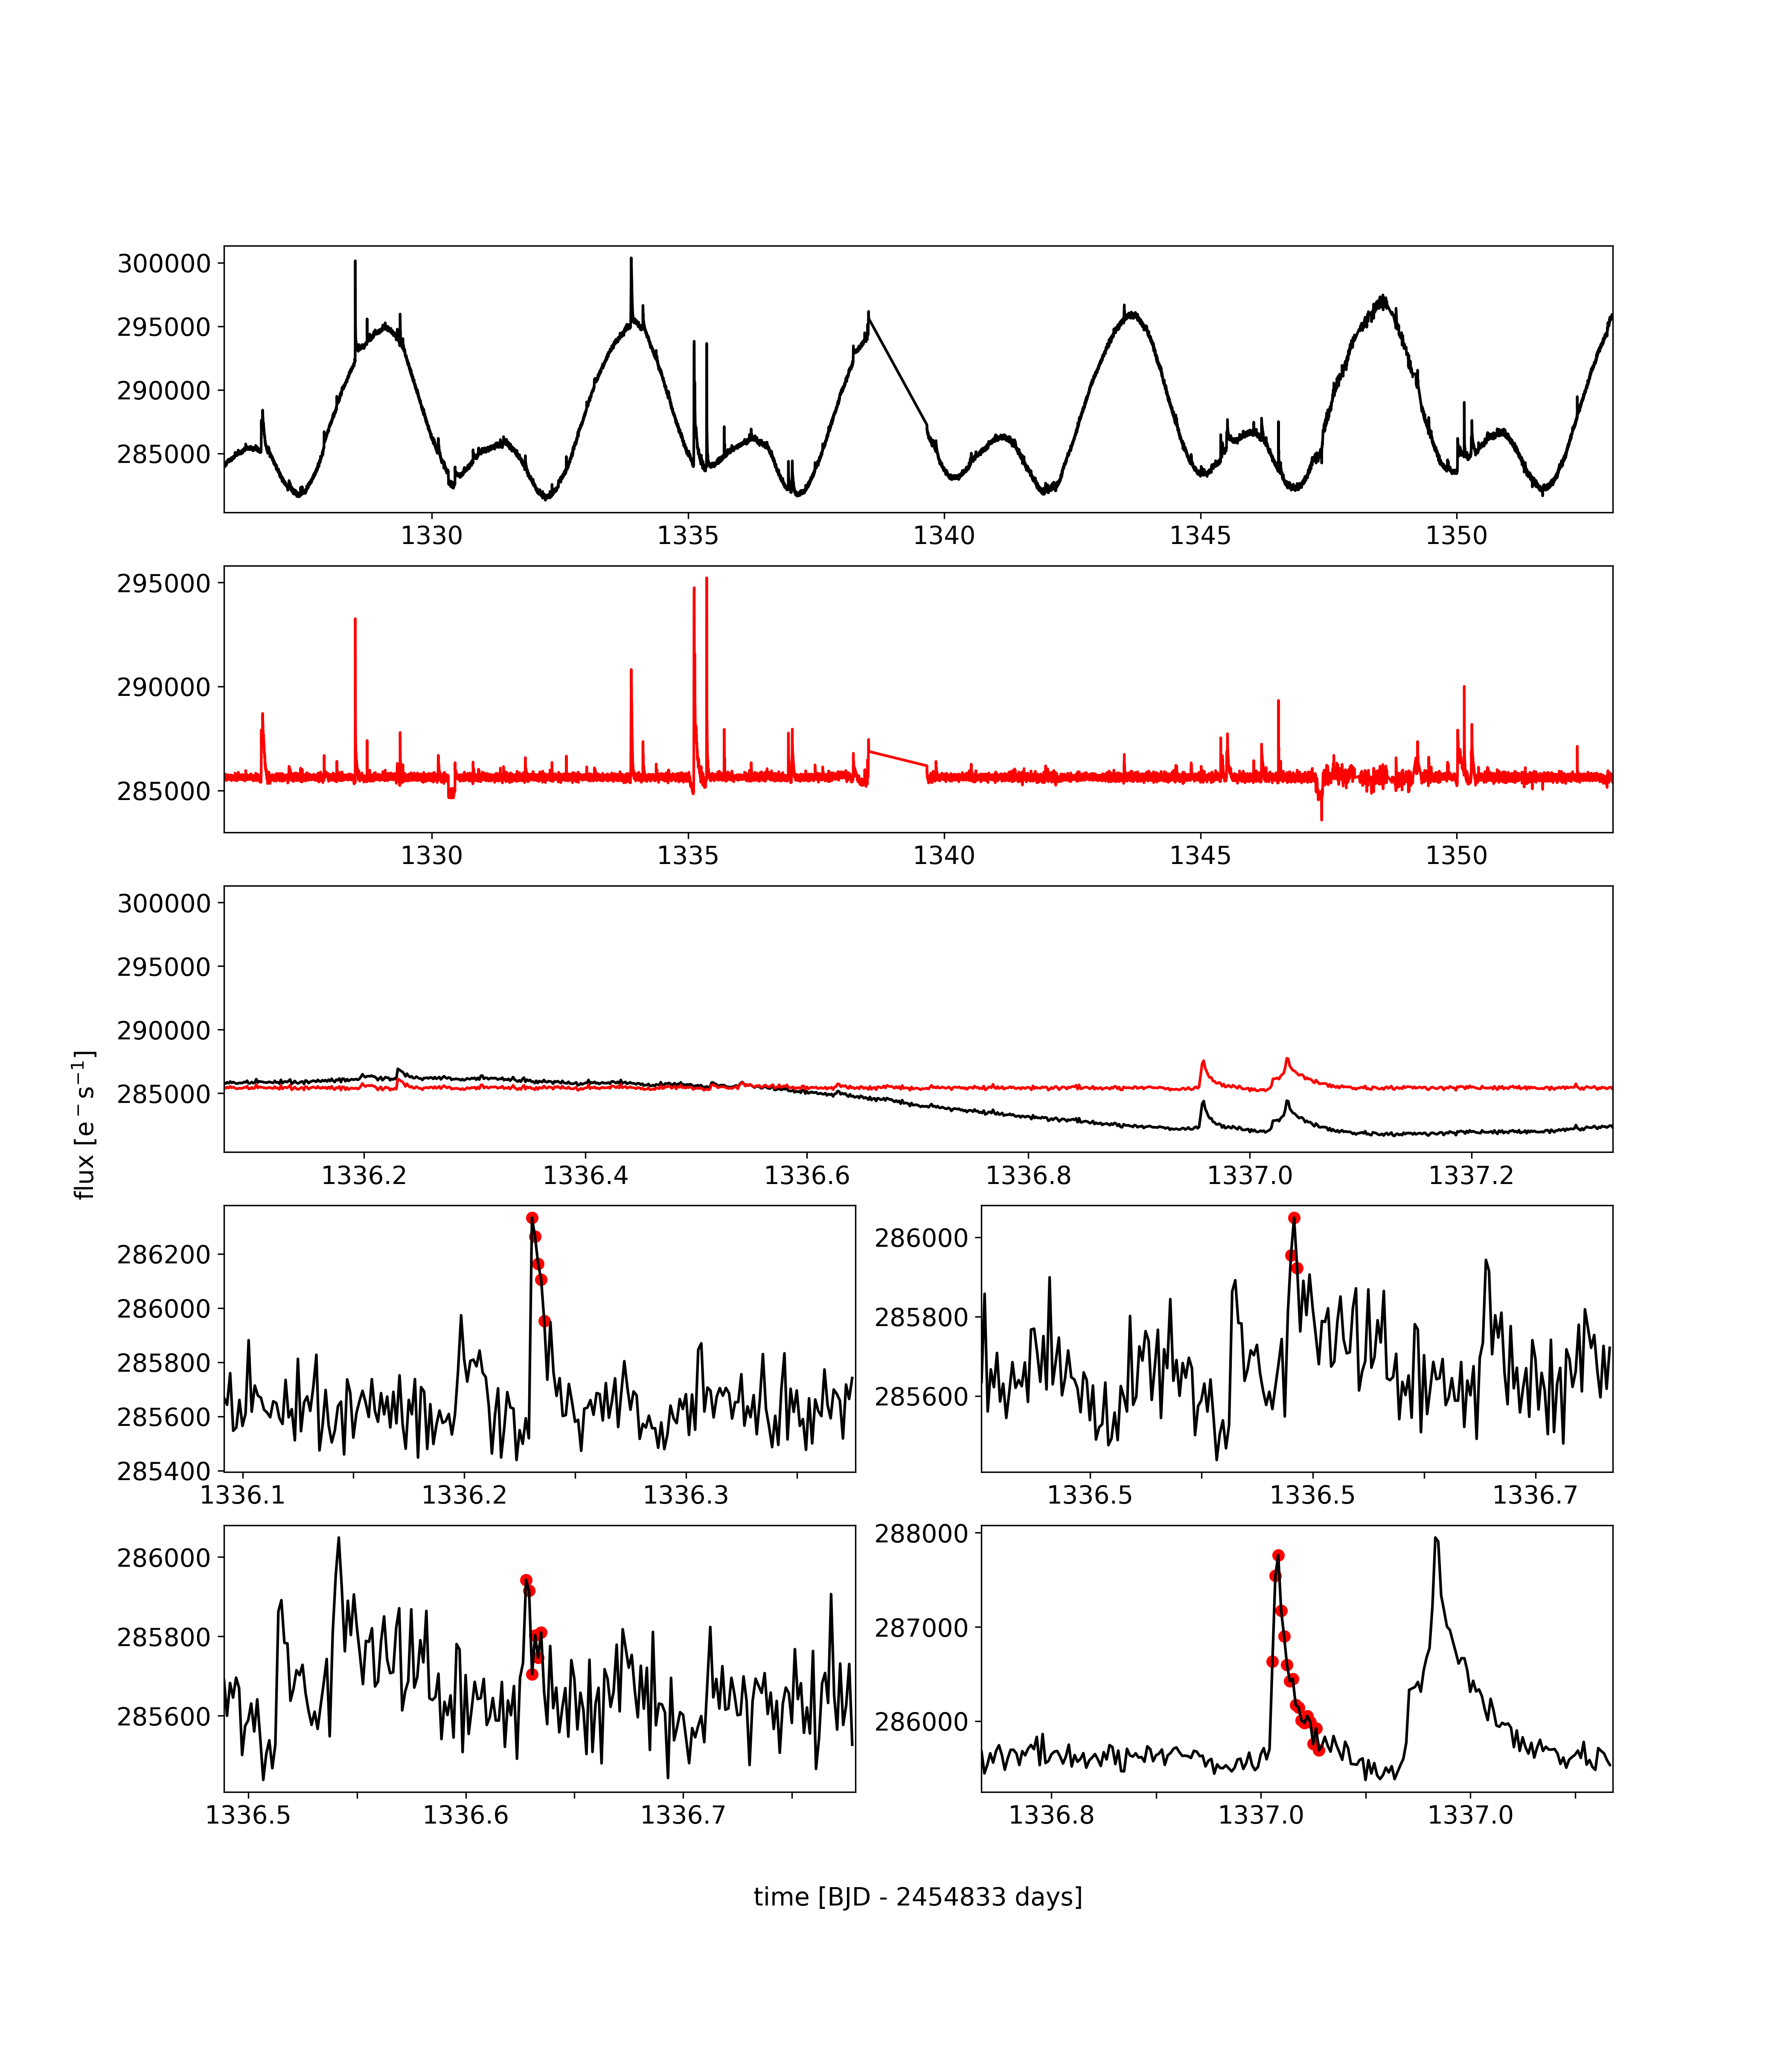
\includegraphics[width=\hsize]{figures/aumic_illustrate_flares.png} 
\caption{Subset of flares detected in the TESS light curve of AU Mic, Sector 1. Top panel: \texttt{PDCSAP\_FLUX} light curve. Second panel from the top: De-trended light curve. Third panel from the top: section from the \texttt{PDCSAP\_FLUX} (black) and de-trended (red) light curve. Four bottom panels: de-trended light curves of flares confirmed in the panel above. The red dots indicate the data points that mark the flares.}
\label{fig:illustrate_detrend}
\end{figure*}

\subsection{Flare catalog}
\label{sec:flarecatalog}
\begin{table}
\caption{Confirmed flare events in the TESS light curves of AU Mic, sorted by orbital phase of AU Mic b. The remainder of the table is available in electronic form.}
\centering
\begin{tabular}{l|ccccc}
\hline
 Sec. &  $t_s$ [BTJD] &  $t_f$ [BTJD] &  orb. phase &    $a$ &         $ED$ [s] \\
\hline
   27 &     2058.2378 &     2058.2526 &       0.001 &  0.007 &  $3.48 \pm 0.04$ \\
   27 &     2058.2584 &     2058.2593 &       0.004 &  0.002 &  $0.10 \pm 0.01$ \\
   27 &     2041.3551 &     2041.3572 &       0.006 &  0.002 &  $0.23 \pm 0.02$ \\
    1 &     1330.4514 &     1330.4709 &       0.007 &  0.003 &  $1.65 \pm 0.03$ \\
   27 &     2041.3690 &     2041.3734 &       0.008 &  0.003 &  $0.70 \pm 0.03$ \\
   27 &     2041.6186 &     2041.6202 &       0.038 &  0.002 &  $0.15 \pm 0.02$ \\
   27 &     2050.1252 &     2050.1259 &       0.043 &  0.003 &  $0.10 \pm 0.01$ \\
   27 &     2050.1724 &     2050.1731 &       0.048 &  0.001 &  $0.07 \pm 0.01$ \\
    1 &     1330.8028 &     1330.8250 &       0.049 &  0.002 &  $1.72 \pm 0.06$ \\
   27 &     2058.7093 &     2058.7148 &       0.057 &  0.004 &  $0.74 \pm 0.03$ \\
\hline

\end{tabular}

\label{tab:flares}
\end{table}

\begin{figure}
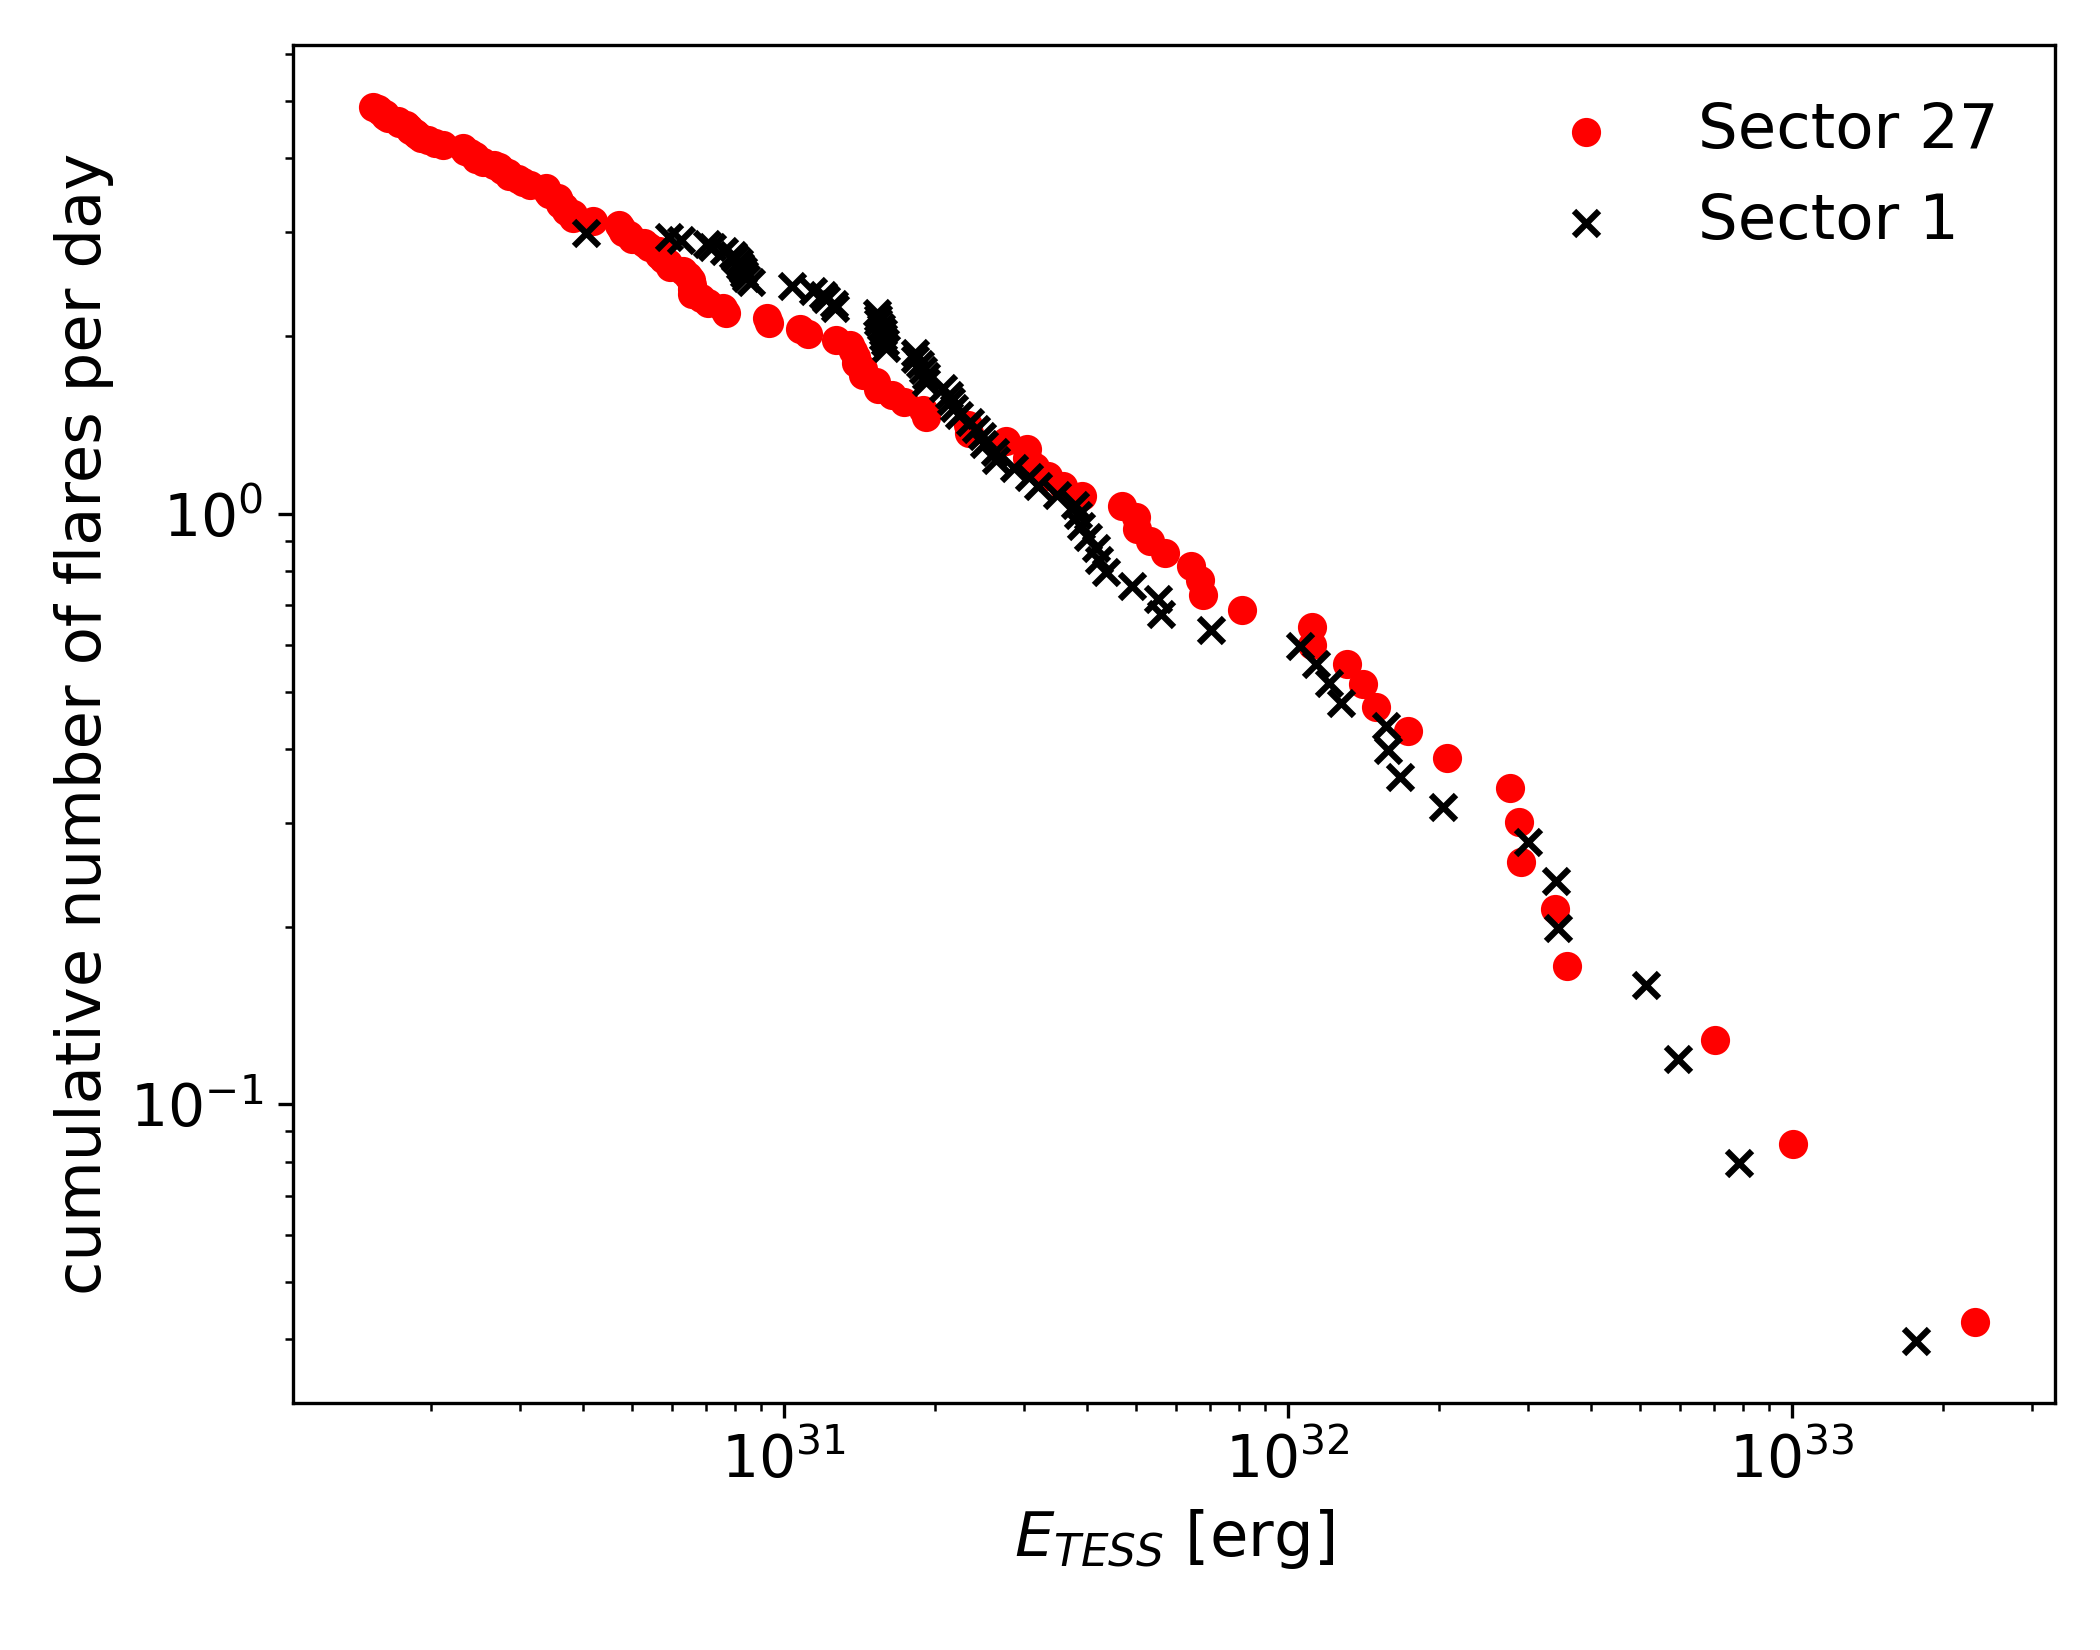
\includegraphics[width=\hsize]{figures/ffd.png} 
\caption{Cumulative flare frequency distributions (FFDs) obtained from the two TESS light curves of AU Mic.}
\label{fig:ffd}
\end{figure}
%We confirmed 75 flares in Sector 1, and 114 flares in Sector 27~(see bottom panels in Fig.~\ref{fig:illustrate_detrend} for examples). We found more flares in Sector 27 because its six times higher observing cadence lowers the detection threshold, which can be seen in the cumulative flare frequency distributions for both Sectors~(Fig.~\ref{fig:ffd}). Overall, we confirmed fewer flares than reported by \citet{martioli2021new} who found the 162 and 157 flares in Sector 1 and 27, respectively. We attribute this difference to the respective detection methods. \citet{martioli2021new} flagged single $2.5\sigma$ outliers as candidates, while we required three consecutive data points $3\sigma$ above the noise. Table \ref{tab:flares} lists the confirmed flare events with their respective start and finish times $t_s$ and $t_f$, orbital phase of AU Mic b at $t_s$, amplitude $a$ and $ED$.
We confirmed 75 flares in Sector 1, and 114 flares in Sector 27~(see bottom panels in Fig.~\ref{fig:illustrate_detrend} for examples). We found more flares in Sector 27 because its six times higher observing cadence lowers the detection threshold, which can be seen in the cumulative flare frequency distributions for both Sectors~(Fig.~\ref{fig:ffd}). Overall, we confirmed fewer flares than reported by \citet{martioli2021new} who found the 162 and 157 flares in Sector 1 and 27, respectively. However, we confirmed almost twice as many flares as \citet{gilbert2021flares}. We attribute these differences to the respective detection methods. \citet{martioli2021new} flagged single $2.5\sigma$ outliers as candidates, while we required three consecutive data points $3\sigma$ above the noise. \citet{gilbert2021flares} used a Bayesian template comparison method to detect probable candidates, which slides a Gaussian rise and exponential decay flare template over the data and returns the probability of belonging to a flare for each data point. Therefore, their method selects flares that fit the template, while we are more senstive to flares that do not conform the classical shape. Table \ref{tab:flares} lists the confirmed flare events with their respective start and finish times $t_s$ and $t_f$, orbital phase of AU Mic b at $t_s$, amplitude $a$ and $ED$.
\section{Flare rate variation with rotational, orbital, and synodic phases}
\label{sec:phases}


%\begin{figure*}
%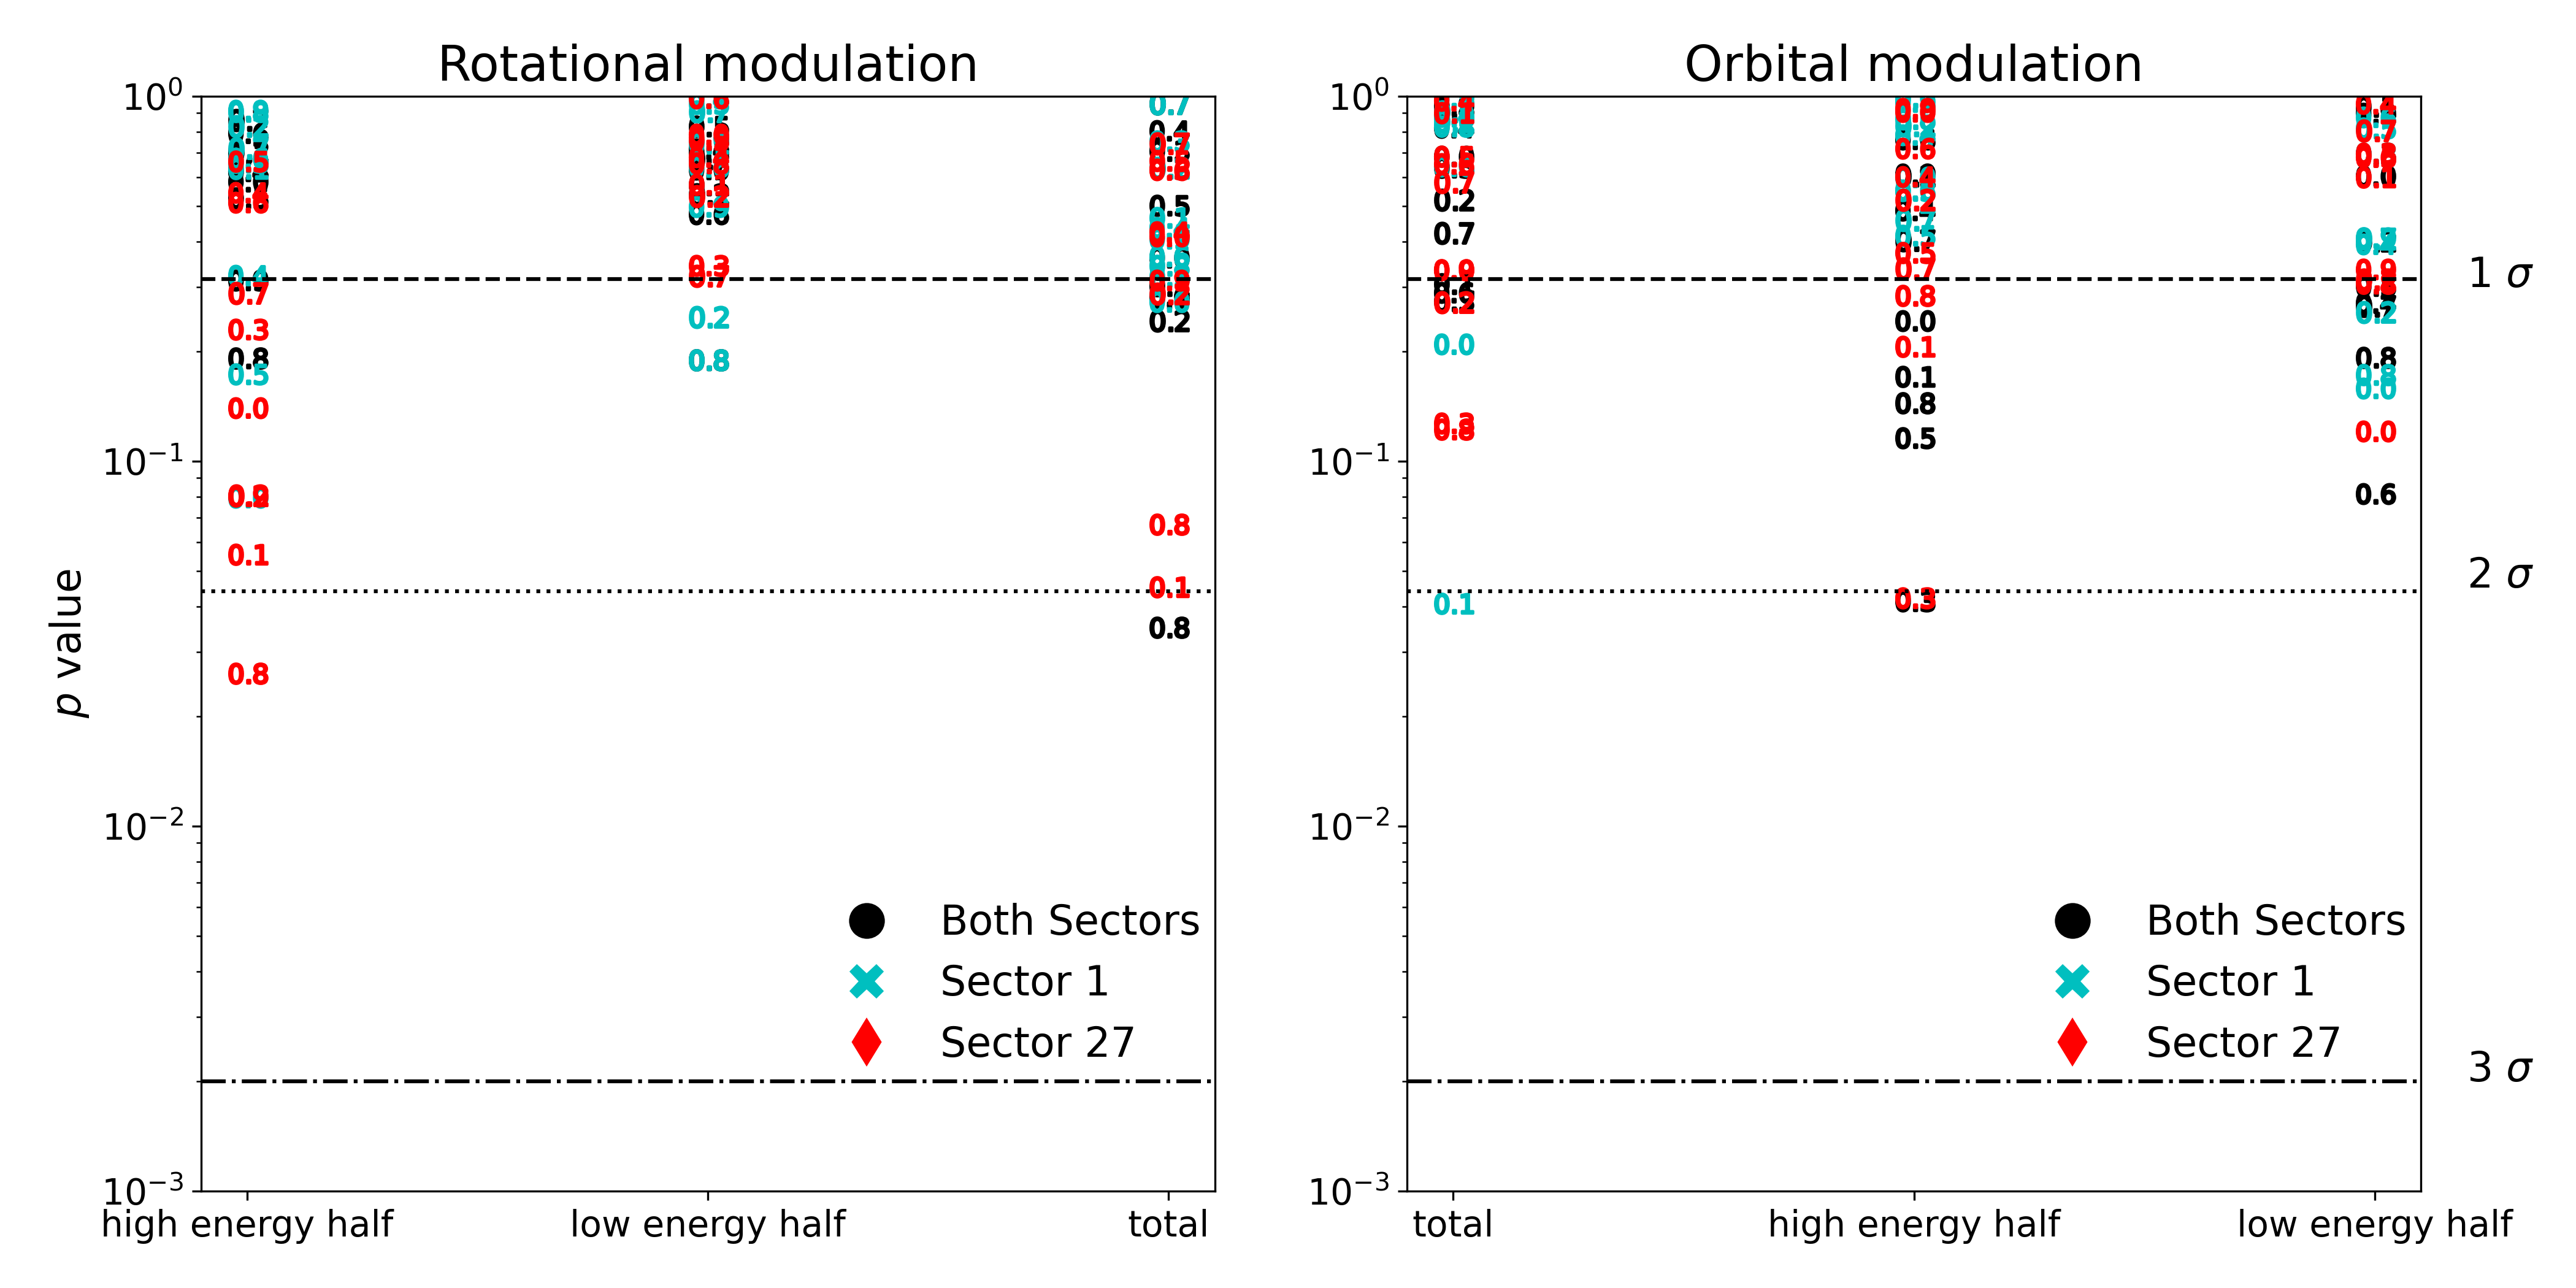
\includegraphics[width=\hsize]{figures/2021_09_01_AUMic_ADtests_meta.png} 
%\caption{Anderson-Darling test results with varying phase offsets.}
%\label{fig:adtest}
%\end{figure*}

\begin{table}
\caption{Mean and standard deviation of $p$ values of the custom AD tests for the orbital, rotational and synodic periods of AU Mic (and AU Mic b) calculated using ten different phase offsets. Smallest $p$-value is boldfaced. There is no significant deviation from uniform flaring in time with either of the periods. $n$: number of flares in sample.}
\centering
\begin{tabular}{llcccc}
\hline
          &  &      & $p(P_{orb})$ & $p(P_{rot})$ & $p(P_{syn})$ \\
sector & sample &     $n$ &              &              &              \\
\hline
both & $ED>1\,$s &   71 &       $\mathbf{0.07}$ &       $0.79$ &       $0.37$ \\
          & $ED<1\,$s &  118 &       $0.52$ &       $0.78$ &       $0.74$ \\
          & total &  189 &       $0.21$ &       $0.57$ &       $0.43$ \\
1 & $ED>1\,$s &   38 &       $0.27$ &       $0.74$ &       $0.48$ \\
          & $ED<1\,$s &   37 &       $0.56$ &       $0.63$ &       $0.44$ \\
          & total &   75 &       $0.20$ &       $0.64$ &       $0.71$ \\
27 & $ED>1\,$s &   33 &       $0.44$ &       $0.10$ &       $0.48$ \\
          & $ED<1\,$s &   81 &       $0.52$ &       $0.53$ &       $0.68$ \\
          & total &  114 &       $0.53$ &       $0.24$ &       $0.68$ \\
\hline
\end{tabular}

\label{tab:pvals}
\end{table}

In analogy to solar flares, stellar flares are thought to occur in the vicinity of active regions on the stellar surface, where magnetic field lines emerge, and magnetic energy can accumulate. AU Mic is a young, extremely active flaring star that is covered with large active regions~\citep{linsky1994, kochukhov2020, plavchan2020}, and possibly a multitude of magnetic loops across the entire corona~\citep{cranmer2013}



Flares on early M dwarfs tend to occur randomly in the various active regions which cover the stellar surface~\citep{doyle2018, doyle2019}. A variation of flaring rate with stellar rotational phase can be caused by an extremely active region on the stellar surface that rotates in and out of view of the observer. A very inactive region that suppresses flaring compared to the rest of the stellar surface is also conceivable, for instance in a region wherein the magnetic field is strong enough to suffiently suppress convection that is required to produce flares. Notably, a non-uniform rotational phase distribution of flares involves only the star. 

When a magentized planet that orbits inside the Alfv\'en surface of the star comes into play, it can introduce a deviation from a uniform flare distribution in time via magnetic star-planet interaction. The magnetic field lines that connect the star's to the planet's magnetic field channel energy from the planet to the star, that is then dissipated via flares. The footpoint of the connection field lines move across the stellar surface as the planet orbit the star. If the stellar properties at the location of these footpoints are negligible in this interaction, excess flares can be observed whenever the footpoint is in view, in phase with the orbital period $P_{orb}$. If, however, the stellar properties at the footpoint's location matter, the occurrence of excess flares will be modulated with the stellar rotation period $P_{rot}$. Then the relevant period is the synodic period $P_{syn}$~\citep{fischer2019}, with

\begin{equation}
P_{syn} = \left|\dfrac{1}{P_{rot}} - \dfrac{1}{P_{orb}}\right|^{-1}.
\end{equation}

In summary, if an inhomogeneous distribution of active regions on the stellar surface, or the interaction of AU Mic with the innermost planet in its orbit takes place that triggers flares in the observable regime, the flaring rates in phase with $P_{rot}$, $P_{orb}$ or $P_{syn}$  will deviate from a uniform distribution. We tested this hypothesis by deriving the expected flaring rate distribution under the assumption that no rotational, orbital, or synodic dependence is present, and comparing it against the observed rate in the TESS light curves. The method is based on the Anderson-Darling test~\citep{anderson1952, stephens2006}:

We analyse $N$ light curves $S_k$ with $k\in [1,N]$ that cover observing periods that do not overlap, and each of which has the same flare detection threshold throughout the observing time of the light curve. It is permissible, however, that this treshold varies from light curve to light curve, as is the case in our data set for AU Mic.
 
After having searched all $S_k$ for flares, we calculate the deviation from a uniform flare rate distribution with orbital, rotational, and synodic phase each using a customized Anderson-Darling test in six steps:
\begin{enumerate}
\item Take all $F$ flare occurrence times from the data and derive their phases $x_i$ with $i \in [1,F]$. 
\item Sort all $x_i$ by phase in ascending order.
\item Calculate observing time per phase using all valid data points in the de-trended light curves, taking into account the different observing cadences.
\item Sample $F$ flare occurrence phases from the phase coverage distribution to get a distribution of flare phases. This step generates a list of flares that are uniformly distributed across all phases.
\item Repeat the previous step to obtain a large number of distributions, and calculate the A-D statistic for each of them.  In this study, we generated 10 000 sample distributions for each test.
\item Finally, compare the A-D statistic of the observed distribution of flare phases against the distribution of A-D statistics from above, and calculate the significance level ($p$-value) of the difference. 
\end{enumerate}

One advantage of the Anderson-Darling test over other flexible test like the Kolmogorov-Smirnov test is its sensitivity to the end of the distribution, i.e. phases near 0 or 1. Since the choice of phase 0 is arbitrary, and the result should not depend on this choice, we performed both the A-D and the K-S test at varying start phases with step size $0.1$. For the A-D test, except for a few outliers, the chosen phases lead to consisent results although there is still some variation at non-significant $p$-values. For the K-S test, the variation with start phase was much larger, yielding both significant and insignificant $p$-values for almost every sub-sample examined. These results demonstrate that neither the A-D nor the K-S test performed on a any single phase starting value can yield definitive answers, but when comparing the two approaches the A-D test is more reliable.

The resulting $p$-values for the A-D test obtained from the above procedure are shown in Table~\ref{tab:pvals}. No choice of Sector, energy split, or period resulted in a consistently significant deviation from uniform flaring in time. 

Because AU Mic is seen nearly equator-on, our results imply a uniform distribution of flares with stellar longitude. The spot structure evolved between Sector 1 and 27~\citep{martioli2021new}, but during each Sector spot patterns were stable over several rotation periods of the star~\citep{szabo2021changing}. However, considering each Sector separately does not reveal any deviation from uniform flaring with longitude. This observation is consistent with most M dwarfs that were searched for rotational periodicity~\citep{doyle2018, doyle2019}. 

The observed distribution of flares does not deviate from a uniform distribution of flares with orbital or synodic period either.  \citet{howard2021evryflare} detected flaring periodicity in 3 out of 284 late K and M dwarfs observed with TESS, and concluded that flaring periodicity might be rare, difficult to detect, or both. 

\section{Discussion}
\label{sec:discussion}

The observed absence of flaring SPI signal can be explained in two ways -- observational biases that impede detection, and physical reasons that prevent flaring SPI to occur in the first place. We consider two physical explanations first.

A first physical reason could be the unknown magnetic field of AU Mic b. It is possible that AU Mic b has no magnetic field that can interact with the stellar magnetic field to trigger flares~\citep{lanza2018close-by}. Planetary magnetic fields in the Solar System are diverse and depend heavily on the internal structure and composition of the planet~\citep{stevenson2003planetary}, and no direct measurements of exoplanet magnetic fields exist today. Therefore, it is difficult to predict the presence, or even the strength of the AU Mic b's field based solely on mass and radius estimates.

Second, AU Mic b's orbit could be outside the Alfv\'en zone of AU Mic, either constantly or temporarily. Although the star has a stron magnetic field, a high mass loss rate may pull the Alfven surface closer to the star~\citep{kavanagh2021}, so that no energy can be channeled from the planet to the star. This situation may change with evolving stellar cycle. \citet{ibanez-bustos2019first} report a 5-year chromospheric activity cycle, but is not clear how it affects mass loss.

Now to the observational biases, of which we discuss three:

First, the effect might simply be too weak. SPI flares may be triggered rarely, with only a handful or fewer of flares in our sample, which are not detectable with sufficient significance. 
%The upper bound on the energies of flares that can arise from the interaction in a handful of sun-like planet hosts is predicted to be well above the detection limit of flares we found in the TESS light curve of AU Mic lanza2018. 

Second, we may be looking into the wrong flare energy regime. Flaring SPI may manifest at low energies $<10^30$ erg, i.e. below the detection threshold. If, on the contrary, the SPI flare regime lies at very high energies, they may again occur too rarely to be observed within the given monitoring time.

Finally, flaring activity could be elevated through flaring SPI, but manifest as excess flares across all longitudes. Efficient transport of the transferred energy in the stellar magnetosphere could even out an interaction that occurs at preferred orbital phases, and can therefore not be distinguished from intrinsically elevated flaring activity.

\section{Conclusions}
\label{sec:conclusions}
Since SPI flares are morphologically identical to intrinsic stellar flares, a statistically significant orbital phase dependence of flaring behaviour is the closest we can currently get to detecting the effect directly. Using high cadence TESS observations of AU Mic, an early M dwarf with a close-in planet detected in 2020, we did not find any sign of flaring SPI.

The strength of the interaction is difficult to constrain in theory~\citep{strugarek2019}, and multiple physical models of flaring SPI co-exist~\citep{lanza2018close-by, saur2013}. Moreover, the orbit of AU Mic b is not yet synchronized with the stellar rotation period which may lead to tidal interaction. Although AU Mic shows the largest number of flares detected among all exoplanet hosts detected to date, we conclude that the vast majority of them are manifestations of intrinsic stellar activity. 

We do not rule out that, as time series observations of AU Mic accumulate with TESS, and soon PLATO~\citep{rauer2014plato}, SPI-triggered flares can be detected. We argue further that long gaps on time scales of months to years betweeen consecutive light curves will may average out rotational variability signal as the spot structure evolves, but should leave a $P_{orb}$-dependent SPI signal intact. 

In an upcoming study, we will apply the methods of flare finding and orbital phase analysis presented here to a large sample of star-planet systems with known close-in planets to increase the total number of orbits covered, and to probe the effects of orbital distance and star-planet mass ratio on the presence and intensity of flaring SPI.
\section*{Acknowledgements}
EI acknowledges support from the German National Scholarship Foundation. KP acknowledges support from the German Leibniz Community under grant P67/2018. We made use of numpy~\citep{numpy2020} and pandas~\citep{pandas2010,pandas2020software}. This research has made use of the SIMBAD database, operated at CDS, Strasbourg, France~\citep{wenger2000}. This paper includes data collected with the TESS mission, obtained from the MAST data archive at the Space Telescope Science Institute (STScI). Funding for the TESS mission is provided by the NASA Explorer Program. STScI is operated by the Association of Universities for Research in Astronomy, Inc., under NASA contract NAS 5-26555.

\section*{Data Availability}
TESS light curves are publicly available through the Mikulski Archive for Space Telescopes (\url{https://mast.stsci.edu/portal/Mashup/Clients/Mast/Portal.html}).
\textcolor{red}{Where shall we store the full flare table?}
%This publication makes use of data products from the Two Micron All Sky Survey, which is a joint project of the University of Massachusetts and the Infrared Processing and Analysis Center/California Institute of Technology, funded by the National Aeronautics and Space Administration and the National Science Foundation.

%This work has made use of data from the European Space Agency (ESA) mission {\it Gaia} (\url{https://www.cosmos.esa.int/gaia}), processed by the {\it Gaia} Data Processing and Analysis Consortium (DPAC, \url{https://www.cosmos.esa.int/web/gaia/dpac/consortium}). Funding for the DPAC has been provided by national institutions, in particular the institutions participating in the {\it Gaia} Multilateral Agreement.
%%%%%%%%%%%%%%%%%%%%%%%%%%%%%%%%%%%%%%%%%%%%%%%%%%

%%%%%%%%%%%%%%%%%%%% REFERENCES %%%%%%%%%%%%%%%%%%

% The best way to enter references is to use BibTeX:

\bibliographystyle{mnras}
\bibliography{bibliography}


% Alternatively you could enter them by hand, like this:
% This method is tedious and prone to error if you have lots of references
%\begin{thebibliography}{99}
%\bibitem[\protect\citeauthoryear{Author}{2012}]{Author2012}
%Author A.~N., 2013, Journal of Improbable Astronomy, 1, 1
%\bibitem[\protect\citeauthoryear{Others}{2013}]{Others2013}
%Others S., 2012, Journal of Interesting Stuff, 17, 198
%\end{thebibliography}

%%%%%%%%%%%%%%%%%%%%%%%%%%%%%%%%%%%%%%%%%%%%%%%%%%

%%%%%%%%%%%%%%%%% APPENDICES %%%%%%%%%%%%%%%%%%%%%

%\appendix
%
%\section{Some extra material}
%
%additional material which would interrupt the flow of the main paper


%%%%%%%%%%%%%%%%%%%%%%%%%%%%%%%%%%%%%%%%%%%%%%%%%%


% Don't change these lines
\bsp	% typesetting comment
\label{lastpage}
\end{document}

% End of mnras_template.tex
